\section{Methods}

\subsection{Data}

Chromosome number data were obtained for all Solanaceae taxa in the the Chromosome Counts Database \citep[CCDB;][]{rice_2015}, and the ca.~14,000 records were cleaned semi-automatically using the CCDBcurator R package \citep{rivero_2019}. % what does "cleaned" mean?
This large dataset includes the compilation of Solanaceae ploidy states from \citet{robertson_2011}.
Species were coded as either diploid (D) or polyploid (P).
For the majority of species, ploidy was assigned according to information from the original publications and the Kew Royal Botanic Gardens C-value DNA resource \citep{bennett_2005}.
For taxa without ploidy information but with information about chromosome number, we assigned ploidy based on the multiplicity of chromosomes within the genus.
For example, \textit{Solanum betaceum} did not include information about ploidy level but it has 24 chromosomes, so because $x=12$ is the base chromosome number of the \textit{Solanum} genus \citep{olmstead_2007}, we assigned \textit{S.~betaceum} as diploid. 
Species with more than one ploidy level were assigned the smallest and most frequent ploidy level recorded.
% E: There was more here about cross-verifying that no P species were SI.  I removed it because there were conflicts before, but we resolved them.  This is addressed in the next paragraph.
%
Breeding system was scored as self-incompatible (I) or self-compatible (C) based on results curated from the literature and  original experimental crosses \citep[as compiled in][]{igic_2006, goldberg_2010, robertson_2011, goldberg_2012}.
Most species could unambiguously be coded as either I or C \citep{raduski_2012}.
Following previous work, we coded as I any species with functional I systems, even if C or dioecy was also reported.
Dioecious species without functional I were coded as C.

%B: It would be nice to clarify what was added--what is new--and separate the subsections of ploidy and breeding system data.
%
% E: I am trying to stick with I/C when talking about the state values, but using SI/SC when talking about the meaning of the trait (because this what people use normally).

To those existing data sets, we added some additional records for chromosome number and breeding system.
The Supplementary Information contains citations for the numerous sources for the added data. % todo: add number of refs when we have it
Resolution of taxonomic synonymy followed the conventions provided in Solanaceae Source \citep{solsource}. %B: was Synonymy followed Solanaceae Source \citep{solsource}.
Hybrids and cultivars were excluded because ploidy and breeding system can be affected by artificial selection during domestication. %B: was: Hybrids and cultivars were excluded because ploidy and breeding system are likely to be altered by domestication.
Following the reasoning outlined in \citet{robertson_2011}, we examined closely the few species for which the merged ploidy and breeding system data indicated the presence of self-incompatible polyploids.
Although SI populations frequently contain some SC individuals, and diploid populations frequently contain some polyploid individuals, in no case did we find a convincing case of a naturally occurring SI and polyploid population.
%B: Thus qualified, as above, I think this should be inserted.
The single instance of an SI and polyploid individual appears to be an allopentaploid hybrid of {\em Solanum oplocense} Hawkes x {\em Solanum gourlayii} Hawkes, reported by \citet{camadro_1981}.
Under exceedingly rare circumstances, it is possible for polyploids containing multiple copies of S-loci to remain SI, so long as they express a single allele at the S-locus (discussed in \citealt{robertson_2011}).
Because of the resulting absence of SI and polyploid populations, as well as the linked functional explanation for disabling of gametophytic self-incompatibility systems with non-self recognition, following whole genome duplication \citep[reviewed in][]{ramsey_1998,stone_2002}, we consider only three observed character states: self-incompatible diploids (ID), self-compatible diploids (CD), and polyploids which are always self-compatible (CP).
%B: I added the non-self recognition bit, because in Prunus, heteroallelic pollen may not cause SC.
% E: Should we include more details about how many polymorphic species and how the particularly tricky ones were dealt with? %B: No and yes, maybe. Interested parties can go to data for part 1?

Matching our character state data to the largest time-calibrated phylogeny of Solanaceae \citep{sarkinen_2013} yielded 595 species with ploidy and/or breeding system information on the tree.
Binary or three-state classification of ploidy and breeding system for the 595 taxa is summarized in \cref{figure:stateclassifications}.
We retained all of these species in each of the analyses below because pruning away tips lacking breeding system in the ploidy-only analyses (and vice versa) would discard data that could inform the diversification models.
A total of 405 taxa without any information about breeding system or polyploidy were excluded.
Tips without trait data are much less informative for diversification parameters linked to trait values.
Including this many more species would have prohibitively slowed our analyses, especially those implementing the most complex models.

% D/P ploidy model
% D/P-A/B ploidy hidden state model
% I/C breeding system model
% I/C-A/B breeding system and hidden state model
% ID/CD/CP ploidy and breeding system model
% ID/CD/CP-A/B ploidy, breeding system, and hidden state model

\subsection{Models for ploidy and diversification}

To investigate the association between ploidy level and diversification, we first defined a binary state speciation and extinction model (BiSSE, \citealt{maddison_2007}) in which taxa were classified as diploid (D) or polyploid (P) (\cref{figure:stateclassifications}).
We call this the D/P ploidy model. 
In a Bayesian framework, we obtained posterior probability distributions of speciation rates ($\lambda_D$, $\lambda_P$), extinction rates ($\mu_D$, $\mu_P$), net diversification rates ($r_D=\lambda_D-\mu_D$, $r_P=\lambda_P-\mu_P$), and relative extinction rates ($\nu_D=\mu_D / \lambda_D$, $\nu_D=\mu_D / \lambda_D$) associated with each state.
This analysis explores the same question as \citet{mayrose_2011, mayrose_2015}, but our analyses differ because we include not only polyploidization (parameter $\rho$, the transition rate from $D$ to $P$), but also diploidization (parameter $\delta$, the transition rate from $P$ to $D$). % E: presumably the motivation will be explained in the Intro

Our second model assesses the the signal of diversification due to ploidy while also parsing out the heterogeneity of diversification rates due a possible unobserved trait.
BiSSE-like models can suffer from a large false discovery rate because they fail to account for diversification rate changes that do not directly depend on the trait of interest \citep{rabosky_2015, beaulieu_2016}.
To allow for diversification rate differences explained by something other than ploidy, we added a hidden state (HiSSE model; \citealt{beaulieu_2016}).
In this model, each of the observed diploid and polyploid states is subdivided by a binary hidden trait with states $A$ and $B$.
We call this the D/P--A/B ploidy and hidden state model. 
We estimated the posterior probability distributions of speciation rates ($\lambda_{D_A},\ \lambda_{D_B},\ \lambda_{P_A},\ \lambda_{P_B}$), extinction rates ($\mu_{D_A},\ \mu_{D_B},\ \mu_{P_A},\ \mu_{P_B}$), net diversification rates ($r_{D_A},\ r_{D_B},\ r_{P_A},\ r_{P_B}$), and relative extinction rates ($\nu_{D_A},\ \nu_{D_B},\ \nu_{P_A},\ \nu_{P_B}$).
In this model polyploidization rate $\rho$ and diploidization rate $\delta$ are also included, and changes between hidden states are symmetrical with rate $\alpha$.

\subsection{Models for breeding system and diversification}

To assess the effects of breeding system in the diversification process, we first fit model in which the states are self-incompatible (I) or self-compatible (C).
This is the same as the analysis of \citet{goldberg_2010}, though with an updated phylogeny \citep{sarkinen_2013}.
We call this BiSSE model the I/C breeding system model. 
To parse out the effect of breeding system in diversification while allowing for the possibility of heterogeneous diversification rates unrelated to breeding system, we subdivided each of those states into hidden states $A$ and $B$.
We call this HiSSE model the I/C--A/B breeding system and hidden state model. 

For these and the subsequent models including breeding system, we allow transitions from $I$ to $C$ (at rate $q_{IC}$) but not the reverse.
Within Solanaceae, self-incompatibility in species that possess it is a homologous form of gametophytic SI \citep[shared even shared even with other dicot families;][]{igic_2001, steinbachs_2002}.
Furthermore, species that are distantly related within the family carry several closely-related alleles at the locus that controls the SI response \citep{ioerger_1990, igic_2006}.
This is very strong evidence that the SI mechanism is ancestral in Solanaceae and has not re-evolved within the family.
% This is an important assumption because ancestral state reconstruction in the models might differ when polyploidy and breeding system are analyzed as independent in the Solanaceae tree.
% This irreversibility assumption prevents self-compatible state from evolving into self-incompatible state and as a result, the ancestral state of all taxa in this model has probability one of being self-incompatible.

\subsection{Models for ploidy, breeding system, and diversification}

If both ploidy and breeding system have the potential to influence lineage diversification, we should logically consider their effects jointly.
We thus fit a model that includes both traits \citep[MuSSE,][]{fitzjohn_2012}.
The three states in this model are self-incompatible diploids (ID), self-compatible diploids (CD), and polyploids, which are always self-compatible (CP).
We did not include a state for self-incompatible polyploids because they are not present in the data, and because that trait combination is logically expected not to occur (as explained above).
We call this the ID/CD/CP ploidy and breeding system model.
It has ten parameters, six for diversification in each state ($\lambda_{ID},\ \lambda_{CD},\ \lambda_{CP}$ for speciation, $\mu_{ID},\ \mu_{CD},\ \mu_{CP}$ for extinction) and four for transitions between states ($\rho_I,\ \rho_C$ for polyploidization transitions from $ID$ and $CD$ to $CP$, respectively; $\delta$ for diploidization from $CP$ to $CD$; $q_{IC}$ for loss of self-incompatibility without polyploidization, from $ID$ to $CD$).
The total rate of loss of self-incompatibility, \ie transitions out of $ID$, is $q_{IC} + \rho_I$.
Diploidization from $CP$ to $ID$ is not allowed because it would be a regain of self-incompatibility.

The ID/CD/CP model could potentially capture similar dynamics as earlier models, if the hidden state in D/P--A/B was effectively breeding system, and the hidden state in I/C--A/B was effectively ploidy.
There is also the potential, however, for a hidden factor to be influencing diversification even beyond both of our focal traits, and this could again mislead inferences.
We therefore added a hidden trait layer on top of our three-state model \citep[analogous to][]{caetano_2018, herrera_2018, huang_2018}.
We refer to this as the ID/CD/CP--A/B model.
A fully parameterized version of this model would have 26 rate parameters \citep{herrera_2018}. 
Because our goal was to look for diversification rate differences associated with ploidy and breeding system rather than the specific effects of the hidden states, we fitted a simplified version with 16 parameters.
The reduction in parameter space is achieved by fixing the rates for transitions among hidden states to be equal with rate $\alpha$, and fixing the transition rates between observed states to be independent of the hidden state (rates $\rho_I,\ \rho_C,\ \delta,\ q_{IC}$ as defined for the ID/CD/CP model).
There are additionally twelve diversification rate parameters ($\lambda_{ID_A},\ \lambda_{ID_B},\ \lambda_{CD_A},\ \lambda_{CD_B},\ \lambda_{CP_A},\ \lambda_{CP_B},\ \mu_{ID_A},\ \mu_{ID_B},\ \mu_{CD_A},\ \mu_{CD_B},\ \mu_{CP_A},\ \mu_{CP_B}$).

\subsection{Diploidization as an exploratory hypothesis}

For all four models that consider ploidy changes, we allowed that diploidization could happen.
Previous modeling approaches \citep{mayrose_2011} have argued against inferring diploidization rates when using ploidy data that comes from classifications based on chromosome number multiplicity or chromosome number change models like chromEvol \citep{mayrose_2010}.
These types of classifications do not allow for a ploidy reversion.
Where indicated, the classification of ploidy for the data used in our models was based on chromosome multiplicity at the genus level.
% ref data/sources table?
However, the majority of the ploidy classifications were adopted from original studies with alternative sources of information (\eg geographic distribution, genus ploidy distribution) where ploidy was defined by authors that found evidence for it.
Since it is not clear whether diploidization can be detected under alternative ploidy classifications or even classifications based on chromosome number multiplicity at the genus level, we also fit the models without diploidization in order to test  whether the conclusions about diversification are sensitive to including diploidization.
As discussed by \citet{servedio_2014}, the presence or absence of a hypothesis can have an exploratory goal.
In our case the diploidization parameter (or its absence, $\delta=0$) in our models is an opportunity to explore an assumption that might be important but that is not the single definitive process to understand the interactions among polyploidy, breeding system, and diversification.

\subsection{Statistical inference under the models}

Parameters for each of the ten diversification models were performed using custom code in the RevBayes \citep{hoehna_2016} environment.
Code and results for all analyses is available at \url{https://github.com/roszenil/solploidy}.
For all analyses, a correction for incomplete sampling was included, based on assuming that the Solanaceae family has approximately 3,000 species ($s=595/3000$) as estimated by the Solanaceae Source project \citep{solsource}.
For all ten models, we assumed that speciation and extinction parameters  had log-normal prior distributions with means equal to the expected net diversification rate $(\text{number of taxa} / [2 \times \text{root age}])$ and standard deviation $0.5$.
Priors for parameters defining trait changes were assumed to be gamma distributed with parameters $k=0.5$ and $\theta=1$. 
For each model, an MCMC chain was run for 96 hours in the high-performance computational cluster at Minnesota Supercomputing Institute, which allowed for 5,000 generation of burn-in and a minimum of 200,000 generations of MCMC for each of the 6 models. 
For each model, convergence and mixing of the MCMC was tested using the R package coda and the software Tracer (see supplementary information for convergence plots). % eventually, add supp info fig ref

\subsection{Model selection}

We calculated the marginal likelihood for each of the ten models in RevBayes \citep{hoehna_2016}.
Marginal likelihoods were calculated using 50 stepping stone steps under the methodology of \citet{xie_2010}.
Each stepping stone step was found by calculating 500 generations of burn-in followed by a total of 1000 MCMC steps (\cref{table:marginallike}).
The calculation of each marginal likelihood ran for 24 hours on a high-performance computational cluster.

Using the marginal likelihood values, we calculated thirteen different Bayes factors. % E: it said "fourteen" but I only count thirteen?
Six compared the models of polyploidy against each other (D/P and D/P--A/B, each with or without diploidization), one compared the breeding system models (I/C and I/C--A/B), and six compared the models with both traits (ID/CD/CP and ID/CD/CP--A/B, each with or without diploidization) (\cref{table:bayesfactors}).
%
Other comparisons between these models are not valid because the input data are different under the different state space codings (\cref{figure:stateclassifications}).
In essence, the D/P, I/C, and ID/CD/CP state spaces are not lumpable with respect to one another \citep{tarasov_2019}.
%R: Emma this is where the figure can be important to show that we have to make different input
% E: I think this short explanation is clear enough, especially with the figure.  I'm not sure whether the hierarchical concept is exactly applicable here.

%\begin{table}
%\begin{tabular}{@{}llccc@{}} \toprule
%\multicolumn{4}{r}{Models} \\ \cmidrule(r){3-5}
%Type & Total of & D/P and D/P-A/B& I/C and I/C-A/B & ID/P/CD and CD/P/ID-A/B\\ \midrule
%Diploid Self Compatible & 152 & 0 &  0 & 0 \\
%Diploid Self Incompatible& 97 & 0  & 1 & 2\\
%Diploid with unknown breeding system & 219 & 0 & (0,1) & (0,2) \\
%Polyploid & 81 & 1& 0 & 1 \\
%Unknow ploidy and self compatible& 34 & (0,1)& 0 & (0,1) \\ 
%Unknown ploidy and self incompatible & 12 & 0 & 1 & 2 \\ \bottomrule
%\end{tabular}
%\caption{Binary and three state classifications for 595 taxa with ploidy and/or breeding system data. The number of taxa in the the sample was maximized by including tips with only ploidy or only breeding system and assigned them as uncertain in the unknown character.}
%\label{table:stateclassifications}
%\end{table}

\begin{figure}
\centering
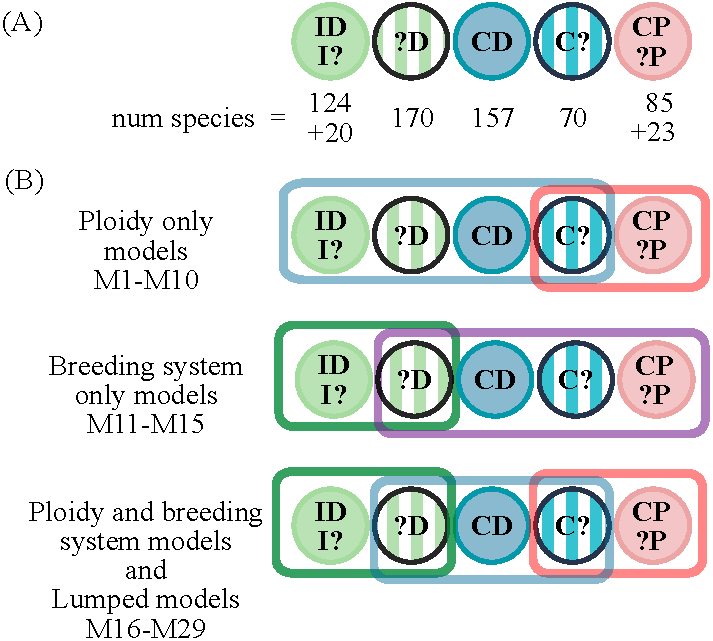
\includegraphics[width=0.5\textwidth]{states.pdf}
\caption{
Character states used for each of the models.
Each species retained on the tree belonged to one of five possible categories, depending on whether ploidy and/or breeding system were known.
The number of species in each is shown under the corresponding circles in the top row.
These categories were then grouped in a manner appropriate to the states of each model.
For example, there are 34 species that are self-compatible and of unknown ploidy; these are coded as either $D$ or $P$ in the D/P models (uncertain, or consistent with either state), as $C$ in the I/C models, and as either $CD$ or $CP$ in the ID/CD/CP models.
In all cases, species were coded as either $A$ or $B$ in the hidden state models.
}
\label{figure:stateclassifications}
\end{figure}


\begin{table}
\begin{tabular}{@{}llcccccc@{}} \toprule
%\multicolumn{4}{r}{Models} \\ \cmidrule(r){3-5}
Model& Model& Ploidy & Diploidization & Breeding  & Hidden & Parameters & Marginal \\
& Type & &  &System & State & & Log- Likelihood \\
1. D/P &BiSSE &	Yes  &	Yes &	No	&No	& 6	& -1182.93 \\
2. D/P no $\delta$ & BiSSE  &	Yes & 	No	& No	& No & 	5 &	-1193.66\\
3. D/P- A/B  & HiSSE &	Yes &	Yes	&No &	Yes &	11 &	\textbf{-1145.69}\\
4. D/P no $\delta$-A/B &	HiSSE &	Yes & No &	No &	Yes &	10	&-1150.99\\
5. I/C &	BiSSE &	No &	 No	&Yes &	No &	 5 &  -1194.80 \\
6. I/C-A/B &	HiSSE &	No &	 No	&Yes &	Yes	& 10 & \textbf{-1155.37}\\
7. ID/P/CD & MuSSE &	Yes & 	Yes &	Yes &	No &	10 & -1344.50\\
8. ID/P/CD no $\delta$ &	MuSSE &	Yes & 	No &	Yes	&No &	9 &-1345.87\\
9. ID/P/CD-A/B & MuHiSSE &	Yes 	&Yes &	Yes &	Yes &	16 & \textbf{-1300.35} \\
10.ID/P/CD no $\delta$-A/B &	 MuHiSSE	 & Yes & 	No	&Yes &	Yes	&15 &-1303.55 \\ \bottomrule
\end{tabular}
\caption{Marginal likelihoods for the ten diversification models proposed.}
\label{table:marginallike}
\end{table}

\begin{table}
\addtolength{\tabcolsep}{-3pt}
\begin{tabular}{|c|c|c|}
\toprule
Polyploidy Models & Breeding System Models & Polyploidy and Breeding System Models \\ \midrule
{\begin{tabular}{lcccc}
 & 1 & 2 & 3 & 4 \\
1. D/P & $\cdot$	 &10.72 &	-37.24	&-31.94\\
2. D/P no $\delta$ &$\cdot$&$\cdot$ &	-47.97	&-42.66\\
\textbf{3. D/P- A/B}  &$\cdot$  & $\cdot$&	$\cdot$	& 5.30 \\
4. D/P no $\delta$-A/B &$\cdot$& $\cdot$ & $\cdot$&$\cdot$ \\
\end{tabular}
}  & 
{\begin{tabular}{lcc}
 & 5 & 6\\
5. I/C &$\cdot$ & -39.43 \\
\textbf{6. I/C-A/B} &$\cdot$& $\cdot$ \\
& & \\
& & \\
\end{tabular}
} & 
{\begin{tabular}{lcccc}
& 7 & 8 & 9 & 10\\
7. ID/P/CD & $\cdot$	&1.36 & -44.15&-40.95 \\
8. ID/P/CD no $\delta$ & $\cdot$ & $\cdot$ & -45.51 &-42.31 \\
\textbf{9. ID/P/CD-A/B}& $\cdot$ & $\cdot$ &$\cdot$	& 3.2 \\ 
10. ID/P/CD no $\delta$-A/B & $\cdot$& $\cdot$&$\cdot$ & $\cdot$\\
\end{tabular}
}\\
\bottomrule
\end{tabular}
 \caption{Bayes factors in log scale. We compare every possible pair. Number models as indicated in  \cref{table:marginallike}. }
\label{table:bayesfactors}
\end{table}



%\begin{tabular}{@{}lcccccccccc@{}} \toprule
%\multicolumn{4}{r}{Models} \\ \cmidrule(r){3-5}
%Model& 1& 2 & 3 & 4  &5 & 6& 7 & 8 & 9 & 10 \\
%Polyploidy & & & & & & & & & \\
%1. D/P &	-  &	10.727 &	-37.243	&-31.941& -	& - & - & - & - &- \\
%2. D/P no $\delta$ & -  & -  &	-47.97	&-42.668& -	& - & - & - & - &- \\
%3. D/P- A/B  & -  & -  &	-	& 5.302 & -	& - & - & - & - &- \\
%4. D/P no $\delta$-A/B &
%Breeding System& & & & & & & & & \\
%5. C/I & -  & -  &	-	& - & -	& -39.434 & - & - & - &- \\
%6. I/C-A/B &
%Polyploidy and Breeding System & & & & & & & & & \\
%7. CD/P/ID & -  & -  &	-	& - & -	& - & - &1.368 & -44.151&-40.951 \\
%8. CD/P/ID no $\delta$& -  & -  &	-	& - & -	& - & - &-& -45.519&-42.319 \\
%9. CD/P/ID-A/B& -  & -  &	-	& - & -	& - & - &-& -& 3.2 \\ 
%10.ID/P/CD no $\delta$-A/B &
%\bottomrule
%\end{tabular}
